\documentclass[10pt,twocolumn,letterpaper]{article}

\usepackage{iccv}
\usepackage{times}
\usepackage{epsfig}
\usepackage{graphicx}
\usepackage{amsmath}
\usepackage{amssymb}
\usepackage{todonotes}

% Include other packages here, before hyperref.

% If you comment hyperref and then uncomment it, you should delete
% egpaper.aux before re-running latex.  (Or just hit 'q' on the first latex
% run, let it finish, and you should be clear).
\usepackage[breaklinks=true,bookmarks=false]{hyperref}

\iccvfinalcopy % *** Uncomment this line for the final submission

\def\iccvPaperID{****} % *** Enter the ICCV Paper ID here
\def\httilde{\mbox{\tt\raisebox{-.5ex}{\symbol{126}}}}

% Pages are numbered in submission mode, and unnumbered in camera-ready
\ificcvfinal\pagestyle{empty}\fi

\begin{document}

%%%%%%%%% TITLE
\title{Detection and Recognition of Dinning Table Objects Using RGB-D Camera for Robotic Applications}

\author{Jakob Baumgartner\\
Faculty of Electrical Engineering,\\
University of Ljubljana\\
Tržaška 25, 1000 Ljubljana, Slovenia\\
{\tt\small jakob.baumgartner@fe.uni-lj.si}
% For a paper whose authors are all at the same institution,
% omit the following lines up until the closing ``}''.
% Additional authors and addresses can be added with ``\and'',
% just like the second author.
% To save space, use either the email address or home page, not both
% \and
% Janez Perš\\
% Faculty of Electrical Engineering,\\
% University of Ljubljana\\
% Tržaška 25, 1000 Ljubljana, Slovenia\\
% {\tt\small janez.pers@fe.uni-lj.si}
}

\maketitle
% Remove page # from the first page of camera-ready.
\ificcvfinal\thispagestyle{empty}\fi

%%%%%%%%% ABSTRACT
\begin{abstract}
In this paper we present a pipeline for 3D segmentation and classification of dining table objects. The created pipeline can be used in real robot applications where we work in an unstructured environment. The algorithm created is able to correctly segment previously seen or unseen objects that might appear on a dining table and classify known common objects. The input to our pipeline is a single RGBD image. We validate our pipeline on an object segmentation database on the table as well as on our own images captured with the Intel Realsense camera.

\todo[inline]{Extend with a couple of more sentences.}



\end{abstract}

%%%%%%%%% BODY TEXT
\section{Introduction}


RGBD (red, green, blue, depth) sensors \cite{Tychola_Tsimperidis_Papakostas_2022} use a combination of traditional RGB (red, green, blue) cameras that capture colour information about an object and depth sensors that measure the distance between the sensor and the object. In the context of a dining table, RGBD sensors can be used to allow the robot to recognise and classify a variety of objects, such as dishes, glasses, utensils and food. By combining the colour information from the RGB cameras with the depth information from the depth sensors, the robot is able to create a detailed 3D model of the objects on the table so that it can recognise their shape, size and orientation.


RGBD object detection and classification algorithms have a number of advantages over traditional object detection algorithms that rely solely on colour information\cite{Rosin_Lai_Shao_Liu_2019}. One advantage of using RGBD information is that the algorithm can better handle occlusion and clutter in the scene. Occlusion occurs when an object blocks the view of another object, and clutter refers to the presence of multiple objects in the scene that may be difficult to distinguish. By using depth information, the algorithm can better understand the spatial relationships between objects and more accurately detect and classify objects even when they are partially occluded or surrounded by clutter. Example of occlusion on a dining table is when a plate is partially hidden behind a glass. Another benefit of using RGBD information is that it enables the algorithm to better distinguish between objects that are similar in colour but different in shape or size. This can be particularly useful when there are multiple objects of the same colour in the scene, as the algorithm can use the depth information to distinguish them based on their shape and size. In our case it can help us distinguish between colourful tablecloths as a background and objects sitting on them. 

However, the use of RGBD object recognition is still less common than the use of RGB object recognition. One reason for this is that RGB sensors are more widespread and less expensive than RGBD sensors. Another reason is the greater difficulty in labelling and especially segmenting such data sets due to the added dimensionality of data. As a result, there are far fewer and less comprehensive RGBD datasets than RGB datasets. For this reason, researchers are trying to train new algorithms on simulated datasets. Such datasets exhibit perfect segmentation, but there is an open problem in transferring the trained models from simulation to working with real data. While synthetic depth trained algorithms usually transfers quite well to real world, simulated RGB images lack the textures and lighting conditions of the real world, so algorithms trained on synthetic RGB data do not transfer well to the real world. This has changed to some extent with the advent of commercial sensors such as Microsoft Kinect and Intel Real-Sense. In addition, algorithms that use RGBD data often require more computing power and resources to analyse the data, which can make them difficult to implement in real-time applications or on devices with limited resources.

In this paper, we aim to create an image processing pipeline that could be used on a robot in the hospitality industry to segment objects on a dining table. We can call this task partially structured because it contains a number of known and unknown objects. A typical input image contains both known objects, such as glasses and plates, and unknown objects, such as items left behind by customers in a restaurant. In order for our robot to clear the table after the guests, it must be able to recognise each object on the table so that it can remove it from the table. We imagine that the robot has three different compartments for the collected items. One compartment for the dirty dishes, one compartment for the rubbish left behind and one compartment for other items, where guests' forgotten items such as wallets and mobile phones are kept, as well as for the tips that guests leave.

In developing this object recognition pipeline, we have paid particular attention to solving challenges that may arise in the dining table environment. In addition to a variety of known and unknown objects, we also deal with objects such as cutlery, napkins and coins that are too thin or too small to be detected in the depth image. Another challenge for this pipeline is the large number of transparent objects such as cups and bottles that commercially available depth sensors cannot detect properly.

%-------------------------------------------------------------------------

\section{Related Work}

In recent years, there has been significant progress in the field of unseen object instance segmentation, which aims to detect and segment instances of objects that have not been seen during training. This is a challenging task that requires the ability to generalize to new objects while still accurately segmenting instances.

Several methods have been proposed to address this problem, including Mask R-CNN by He et al. (2017) \cite{He_Gkioxari_Dolla\textbf{\textbf{}}r_Girshick_2018} \cite{Danielczuk_Matl_Gupta_Li_Lee_Mahler_Goldberg_2019}, which extends the Faster R-CNN framework to predict instance masks in addition to object bounding boxes. Panoptic FPN by Kirillov et al. (2019) \cite{Kirillov_Girshick_He_Dollar_2019} also builds upon the FPN architecture to generate panoptic segmentation, including both object instances and stuff segments. YOLACT by Bolya et al. (2019) \cite{Bolya_Zhou_Xiao_Lee_2019} uses a fully-convolutional model, that trades some of the segmentation performance for being able to run real-time. 
SolO-instance by Wang et al. (2020) \cite{Wang_Kong_Shen_Jiang_Li_2020} uses a set of prototypes to represent object instances, which are then refined in a manner that allows for instance-specific predictions. PointRend by Kirillov et al. (2020) \cite{Kirillov_Wu_He_Girshick_2020} uses a neural network module that performs point-based segmentation predictions at adaptively selected locations based on an iterative subdivision algorithm. PointRend achieves significantly better segmentation results on several popular datasets compared to previous approaches. PolarMask by Xie et al. (2020) \cite{Xie_Sun_Song_Wang_Liang_Shen_Luo_2020} introduces an anchor-box free and single-shot instance segmentation method that can be used as a mask prediction module for instance segmentation. PointGroup by Jiang et al. (2020) \cite{Jiang_Zhao_Shi_Liu_Fu_Jia_2020} presents a new end to-end bottom-up architecture, specifically focused on better grouping the points by exploring the void space between objects. 

The following methods focus specifically on the segmentation of unseen instances. In the absence of sufficiently large datasets for segmenting instances in cluttered environments, these approaches use synthetic data and generalise the algorithms so that they are applicable to the detection of real-world data \cite{Xie_Xiang_Mousavian_Fox_2020}. These methods are most comparable to our method of choice, which is also trained on synthetic data. Being state-of-the-art, these methods offer similar performance to the method we chose for segmentation, while working at the same speed or slower. UCN by Xiang et al. (2021) \cite{Xiang_Xie_Mousavian_Fox_2021} uses RGB-D feature embeddings from synthetic data to perform instance segmentation. MSMFormer by Lu et al. (2022) \cite{Lu_Chen_Ruozzi_Xiang_2022} uses a new transformer architecture that simulates the von Mises-Fisher (vMF) mean shift clustering algorithm.

These methods demonstrate the progress that has been made in unseen object instance segmentation and highlight the potential for future developments in this field.


\section{Methods}


\begin{figure*}
\begin{center}
  \makebox{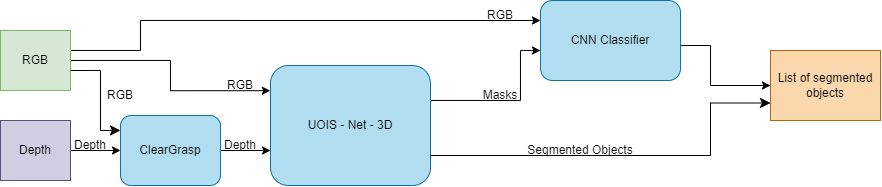
\includegraphics[width=0.75\paperwidth]{structure-graph.png}}
\end{center}
   \caption{Full proposed pipeline. \todo[inline]{Remove clearGrasp from image}}
\label{fig:structure-graph}
\end{figure*}



% overview
Our pipeline consists of two separate components, as can be seen in the figure \ref{fig:structure-graph}. Together, they allow us to solve the problem of instance segmentation and classification of objects on a dinner table in a real-world environment. The input to our pipeline is a single RGB-D image. Our method returns a list of segmented instances with segmentation masks and the positions of the objects. Our method also returns classifications for objects that are common in the given environment.

The first component in our pipeline is an Unseen Object Instante Segmentator (UOIS) \cite{Xie_Xiang_Mousavian_Fox_2021}. Due to the unstructured nature of our task, it is infeasible and impractical to model every possible object in our environment. For a robot to successfully manipulate objects on a dining table, it must be able to recognise and segment instances of previously seen and unseen objects \cite{Xie_Xiang_Mousavian_Fox_2020}. This component takes as input RGB and point cloud data and provides segmentation masks and positions for each known and unknown object on the dining table. It is able to segment objects even if they are cluttered together or partially occluded. Before we can use this stage, we need to backproject Depth image back onto the point cloud data \cite{Bostanci_Kanwal_Clark_2015}, for this we need to know the intrinsic matrix of the camera used.

The second component of our pipeline is a CNN classifier. UOIS provides instance segmentation masks. With these, we can cut out individual objects and then perform a classification for the common objects on a dining table. These detections can be passed on to the robot so that it can separate kitchen utensils such as plates, cups and cutlery from other objects and the rubbish left on the table.


% UOIS

\subsection{Unseen Object Instance Segmentator}

To divide cluttered objects on the dining table into individual instances, we use Unseen Object Instance Segmentator (UOIS-Net-3D) \cite{Xie_Xiang_Mousavian_Fox_2021}. The algorithm takes as input a single RGBD image and outputs object instance segmentation masks for all previously seen or unseen objects. The output of the algorithm does not contain specific categories of objects, only background, table and object instance.

The algorithm consists of separately trained neural networks and multiple stages. A simple representation of the algorithm can be seen in the figure \ref{fig:UOIS-scheme}.

\begin{figure}
\begin{center}
     \makebox{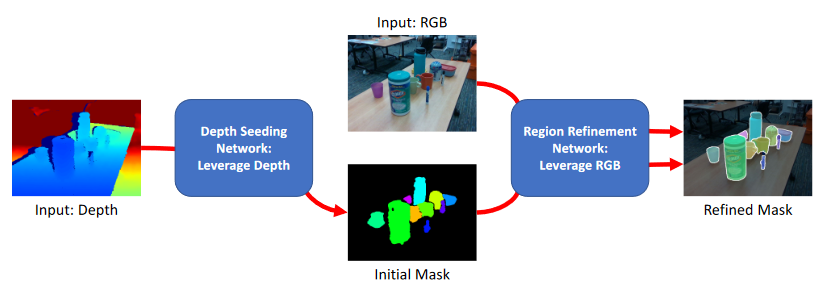
\includegraphics[width=1\linewidth]{UOIS-scheme.png}}
\end{center}
   \caption{UOIS-Net-3D consists of two neural networks, that process Depth and RGB data seperately, to produce instance segmentation masks.}
\label{fig:UOIS-scheme}
\end{figure}

\begin{figure}
\begin{center}
     \makebox{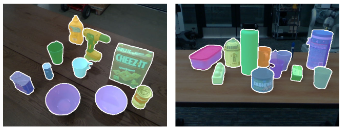
\includegraphics[width=1\linewidth]{UOIS-examples.png}}
\end{center}
   \caption{We use UOIS-Net-3D algorithm to segment all objects in the image.}
\label{fig:UOIS-example}
\end{figure}

\subsubsection{Method}

\textbf{Depth Seeding Network - DSN}
The first stage of the instance segmentation network takes as input an organised point cloud D with XYZ coordinates. The reason why we use depth data first is because of the better generalisation of neural networks trained on simulated depth data to real-world scenarios, compared to networks trained on synthetic RGB data. The organised point cloud is passed through the DSN network, which returns a segmentation mask for each pixel for the given image and the 3D offsets to the object centres. \(V'\in\ \Re^{H \times W \times 3}\).

\textbf{Initial Mask Processing Module - IMP }
In this phase of the algorithm, we apply some basic image techniques to the initial segmentation mask. First, we apply an opening operation (erosion+dilation) to each mask instance to remove salt/pepper noise. Then we apply a closing operation (dilation+erosion) to remove small holes in the mask. Finally, we remove minor unconnected components of each mask. 

\textbf{Region Refinement Network - RRN}
At this stage, we use another neural network to refine the segmentation mask obtained from the depth image with additional RGB information. The input of the RRN is a 4-channel cropped image consisting of a concatenated cropped RGB and a single object mask. We use a U-Net \cite{u-net} network architecture.
During the training process, we first train the DSN network and then use the output segmentations for RRN training. During training, we first use the segmentation masks before input to the RRN. This allows us to simulate the noise and errors that occur when using data from a real depth sensor but are not seen on the clear synthetic images. For pertrubation, we use augmentation techniques such as translation, rotation, addition, cutting, morphological operations and random elipses. For an example of a segmentation result, see image \ref{fig:UOIS-example}. 

\subsubsection{Dataset}
The method was trained on a synthetic dataset called the Tabletop Object Dataset (TOD). The dataset consists of 40,000 synthetic scenes. Each scene consists of a SUNCG \cite{Song_Yu_Zeng_Chang_Savva_Funkhouser_2016} home environment. In this environment is a ShapeNet \cite{Chang_Funkhouser_Guibas_Hanrahan_Huang_Li_Savarese_Savva_Song_Su_et} model of a table with 5 to 25 ShapeNet \cite{Chang_Funkhouser_Guibas_Hanrahan_Huang_Li_Savarese_Savva_Song_Su_et} models of objects randomly placed or stacked on the table. For each object, the constalation dataset contains seven different views. Due to the limitations of the simulator used (PyBullet), RGB textures do not look photorealistic. The depth data, while clear compared to data from an actual commercial sensor, is closer to a realistic representation.A synthetic dataset was used as there is no dataset collected and annotated in the real world that meets the requirements for training such an application.

\todo[inline]{Move Datasets into its own section}

% CNN

\subsection{Classifier}
The final component of our pipeline is an image classification network. We use segmentation masks obtained from UOIS to cut out each object from the RGB image and then use the ResNet \cite{He_Zhang_Ren_Sun_2015} convolutional model to classify each object into one of the categories listed. The categories are: Cup, Plate, Bowl, Glass, Cutlery, Purse, Napkin, Tin, Bottle, Other. The idea behind this is that a robot working in the hospitality industry can divide the objects into a section for laundry and a section for the bin / other objects.

\textbf{Dataset}
To train our classifier, we used images from the ImageNet dataset for the specified categories. ImageNet consists of more than 20,000 categories, but we selected for training only images from the categories we chose and a set of images with random objects to train the so-called "other" category. Half of the images we selected are from objects we want to classify and the other half of the images are from a number of different uncategorised objects.

\todo[inline]{Correct data about dataset used for training.}

% Hardware

\section{Experiments}
In order for our pipeline to be useful for robotic applications, it must be able to work with a high success rate in each part of the pipeline and execute at a reasonable speed. In the experimental part of this article, we therefore focus on testing parts of the pipeline individually and in conjunction with others.

To perform the experiments, we have created the pipeline of algorithms described. We use PyTorch \cite{Paszke_Gross_Massa_Lerer_Bradbury_Chanan_Killeen_Lin_Gimelshein_Antiga_et} implementations \cite{UOIS-git} \cite{resnet-Pytorch} of each of the methods described above. To avoid problems with different versions of PyTorch as well as other dependencies, we run each of the components in a separate Docker container.

The experiments were conducted on a computer with Intel® Core™ i7-12700 CPU,
GEFORCE GTX 1080 Ti GPU and 32GB of RAM performed.

\subsection{Object Segmentation Database (OSD)}

Our experiments can be divided into two parts. First, we tested our system with the Object Segmentation Database (OSD).

We perform an ablation experiment to see how removing the augmentation network for transparent objects at the beginning of the pipeline affects the segmentation and classification results. The purpose of this test was to see if using augmented data affects the segmentation of non-transparent objects in any way.

We test how accurate our classifier is.

We also measure the time it takes each of the pipeline components to perform computations. We pay attention to how the number of opaque objects affects the computation times.

\subsection{Intel RealSense D435}

In the second part of the experiments we use the Intel RealSense D435 camera to capture a series of RGBD images. The goal of this experiment is to see if our pipeline works on new data. Besides general examples, we use the camera to capture several RGBD images of situations that are not included in the OSD database.

We take 25 different images that contain transparent objects. We then compare the results of segmenting transparent objects with and without using the ClearGrip component to enhance the depth images.

Then we take a series of images of small and thin objects. The RGBD camera has a resolution of 2\% error at distances of less than 1m. This means that certain small or thin objects are not visible on the depth image. Examples of such objects are cutlery, paper pages or menus. We want to test whether the segmentation algorithm used can recognise these objects based on RGB data alone. Since the first detection step in the UOIS uses depth information, we expect that these objects will not be detected.

\section{Experiments}
\todo[inline]{Add section}

\subsection{Hardware}
To deploy our algorithm, we would need adequate hardware. Deep neural nets can be computationally intensive, and to run them efficiently, a lot of processing power is required. GPUs, are designed particularly for parallel processing and are well-suited for this task, as they can perform multiple mathematical operations simultaneously. We utilized cloud GPUs from Google Colab tool for testing, using the Tesla T4 with 16GB of memory and 13GB of system RAM. This is a GPU, manufactured by Nvidia, that is specifically designed for deep learning.


\subsection{Time trials}

We have imagined an application that is intended to operate on a robot that moves in a changing environment. Consequently, our pipeline must be capable of operating in real-time, with as many frames per second as possible. In this part of the experiments, we separately tested our segmentator and classifier, and then together to determine how many images per second our pipeline is capable of processing.

\todo[inline]{add results, add table}

\section{Results}
\todo[inline]{Add section}
\todo[inline]{mention failure modes (small objects, transparent objects and light conditions)}


% UOIS-3D-Net

% MaskRCNN - can I train this?!? dataset err

% Klasifier

% Time

% Dataset






{\small
\bibliographystyle{ieee_fullname}
\bibliography{egbib.bib}
}

\end{document}
